% IEEE conference paper template for kaggle2 KIE pipeline comparison
% Compile: pdflatex paper_filled.tex && bibtex paper_filled && pdflatex paper_filled.tex
% Sections live under sections/ and are inlined by ``report.inject.expand_inputs``
% before the Python substitution pass, so tectonic sees a single flat .tex.
\documentclass[conference]{IEEEtran}
\usepackage{cite}
\usepackage{amsmath,amssymb}
\usepackage{graphicx}
\usepackage{booktabs}
\usepackage{tikz}
\usetikzlibrary{arrows.meta,positioning,fit,backgrounds}

\begin{document}

\title{End-to-End vs.\ Pipeline Receipt KIE:\\
       DONUT Against YOLO+TrOCR+Attention on SROIE}

\author{\IEEEauthorblockN{Anonymous}
\IEEEauthorblockA{Under review}}

\maketitle

\begin{abstract}
We compare two architectures for Key Information Extraction (KIE) on
the SROIE receipt benchmark (500\,/\,63\,/\,63 train\,/\,val\,/\,test
split): an end-to-end sequence-to-sequence model (DONUT,
$\approx$200\,M parameters) and a modular detect-then-read pipeline
(YOLOv8\,$+$\,TrOCR\,$+$\,learned attention assigner).
Training on 500 receipts, DONUT achieves a global token-F1 of
0.7905 and the pipeline achieves 0.7912
($\Delta$F1\,=\,-0.0007, within single-seed noise).
Our attention assigner --- a $\approx400\,$K-parameter
Transformer-encoder\,$+$\,cross-attention module with four learned
field queries, 6-d handcrafted text priors, and a multi-instance
negative-log pos-mass loss --- closes the gap over rule-based
assignment by 0.1103 absolute F1 points, while
producing per-field attention maps that are interpretable by inspection,
a property the monolithic DONUT architecture cannot offer.
We document thirteen previously unreported implementation bugs that
silently destroy F1, characterise the address field's structural failure
mode in pipeline systems, and publish GPU telemetry alongside every
reported number (24\,GB peak VRAM,
0.2808\,USD per DONUT run on a vast.ai RTX\,4090).
\end{abstract}

\section{Introduction}

Receipt Key Information Extraction (KIE) --- recovering structured
fields such as merchant name (company), date, address, and total amount
from scanned or photographed receipts --- underpins tax-audit
automation, expense management, and digital accounting at scale.
The SROIE benchmark~\cite{huang2019icdar}, introduced at ICDAR~2019,
has become the standard testbed for this problem: 626 labelled receipt
images from East Asian and Southeast Asian vendors, with four
ground-truth text fields per image and character-level bounding-box
annotations.

Two paradigms have emerged for solving KIE.
\emph{End-to-end vision-language models}, exemplified by
DONUT~\cite{kim2022donut}, treat the entire receipt image as a sequence
of visual patches and autoregressively decode structured text without an
explicit OCR stage.  The appeal is simplicity: a single forward pass
produces all field values from pixels, and no handcrafted feature
engineering is required.  The cost is opacity: there is no intermediate
variable one can inspect to understand \emph{why} a prediction was made,
and every parameter --- including the large majority that never fire on
any given receipt --- is carried through every forward pass.
\emph{Pipeline systems} decompose the problem: a text detector
(YOLOv8~\cite{jocher2023yolov8}) finds and crops text lines;
an OCR model (TrOCR~\cite{li2023trocr}) reads each crop;
and a field assigner maps the resulting text tokens and bounding boxes
to the target schema.  Pipelines are interpretable --- each stage
produces an auditable intermediate representation --- and fast to
iterate: retraining the $\approx400\,$K-parameter
assigner takes minutes, whereas
retraining DONUT from a new base takes hours.
At roughly half the end-to-end parameter cost of DONUT, the analytical
route with a learned cross-attention assigner effectively \emph{discards
the unused parameters} DONUT carries: the heavy perceptual work is
delegated to YOLOv8 (a parametrically cheap detector) and TrOCR (a
crop-level OCR decoder), while the $\approx400\,$K
attention assigner concentrates its capacity on the single hard problem
of line-to-field assignment.  This re-budgeting is the central
efficiency argument we make on SROIE.

The central question this paper asks is: \emph{can a lightweight
learned assigner close the F1 gap between an end-to-end model and a
pipeline, and at what interpretability cost to each?}  We answer this
question on the SROIE dataset with a fixed 500\,/\,63\,/\,63
train\,/\,val\,/\,test split, no validation leakage, and a fixed seed (42).

\medskip
\noindent\textbf{Contributions.}
\begin{enumerate}
\item A like-for-like comparison of DONUT and a detect-then-read
  pipeline at a fixed data budget of 500 training receipts, with
  bootstrap 95\,\% confidence intervals and McNemar's test to
  characterise statistical significance on the small test set.
\item A $\approx400\,$K-parameter
  Transformer-encoder\,$+$\,cross-attention assigner with four
  learned field queries (\texttt{company}, \texttt{date},
  \texttt{address}, \texttt{total}), 6-d handcrafted text priors,
  and a multi-instance negative-log pos-mass loss; published with
  reproducible code, a fixed data split, and seed 42.\footnote{The repo's
  architectural discipline --- 166-LOC cap, 2-in/1-out function
  contracts, flat module layout, and mypy --strict as the test suite
  --- is adapted from the C99 companion project
  \texttt{aiparallel0/teb2}, ensuring every module is individually
  auditable.}
\item A catalogue of thirteen silent F1-destroying implementation bugs
  found during development, with symptom, mechanism, and guard for
  each.
\item Full GPU telemetry (utilisation, memory, power, temperature,
  cost, CO$_2$eq) published alongside F1, following the honest-benchmark
  framing of~\cite{strubell2019energy}.
\end{enumerate}


\section{Related Work}

\subsection{End-to-End Document Understanding}
DONUT~\cite{kim2022donut} eliminates OCR entirely: a Swin
Transformer~\cite{liu2021swin} encodes image patches and a BART-style
decoder~\cite{lewis2020bart} autoregressively emits structured JSON
wrapped in XML-style tags.  Dessurt~\cite{davis2022dessurt} follows a
similar paradigm with a different pre-training task.
Pix2Struct~\cite{lee2023pix2struct} parses screenshots, charts, and
documents from variable-resolution patches.  These models scale
strongly with data but are expensive to retrain and produce no
interpretable intermediates.

\subsection{Pipeline and Hybrid KIE}
LayoutLM~\cite{xu2020layoutlm} and LayoutLMv3~\cite{huang2022layoutlmv3}
fuse OCR tokens with 2D positional embeddings in a BERT-style encoder;
they require an upstream OCR step and post-processing to assign tokens
to fields.  CUTIE, PICK, and GCN-based approaches treat KIE as node
classification on a document graph whose nodes are OCR-detected text
regions.  BROS~\cite{hong2022bros} adds relative spatial attention.
Compared to end-to-end models these pipelines excel in low-data
regimes and offer interpretable intermediate representations at the
cost of error accumulation across stages.

\subsection{Receipt Benchmarks}
SROIE~\cite{huang2019icdar} (626 receipts, 4 fields, ICDAR~2019) is
the standard single-vendor-type benchmark.  CORD~\cite{park2019cord}
covers Korean restaurant receipts with a richer 30-field ontology.
WildReceipt~\cite{sun2021wildreceipt} extends to in-the-wild image
conditions.  RVL-CDIP targets document classification rather than KIE.
We restrict experiments to SROIE because it is the most studied and
because our predecessor work~\cite{aiparallel0kaggle} characterised
its multi-dataset oversampling dynamics.


% -----------------------------------------------------------------------
% Methodology section: dataset, splits, DONUT baseline.
% Project: kaggle2 — End-to-End vs. Pipeline Receipt KIE on SROIE.
% Role: top-level Methodology section; the YOLO+TrOCR+Attention pipeline
%   subsection is split into method_pipeline.tex to honour the 166-LOC
%   per-file cap.
% -----------------------------------------------------------------------

\section{Methodology}

\subsection{Dataset and Splits}
We use all 626 SROIE images with a deterministic seed-42 shuffle:
500 train\,/\,63 validation\,/\,63 test.  The split is computed once
and persisted to \texttt{results/split.json} so that no image can
appear in both validation and test sets (Bug~7 in Section~\ref{sec:bugs}).

\subsection{DONUT: End-to-End Vision-to-Text}

DONUT~\cite{kim2022donut} fine-tuned from \texttt{naver-clova-ix/donut-base}
is our end-to-end baseline.  The architecture is a Swin
Transformer~\cite{liu2021swin} encoder that processes the receipt image
as non-overlapping $4{\times}4$ patches through a hierarchical
shifted-window attention pyramid (so both ``top-of-receipt'' and
``near-bottom-total'' are representable without explicit coordinates),
followed by a BART decoder~\cite{lewis2020bart} that
autoregressively emits structured output wrapped in XML-style task tokens.

\textbf{Autoregressive XML decoding.}
The decoder is conditioned on a task prompt
\texttt{<s\_sroie>} and emits tokens until it produces
\texttt{</s\_sroie>}.  A well-trained DONUT generates output of the form:
\texttt{<s\_company>SUPER MART</s\_company><s\_date>03/01/2019}
\texttt{</s\_date><s\_address>NO.~1 JALAN~...</s\_address>}
\texttt{<s\_total>43.50</s\_total>}.
The \texttt{token2json} helper then parses the XML to a Python dict
(after flattening any outer \texttt{sroie} wrapper key; Bug~12).

\textbf{Differential learning rate.}
We train the decoder at $5{\times}10^{-4}$ and the encoder at
$5{\times}10^{-5}$ --- a 10$\times$ ratio.  The decoder's embedding
matrix is \emph{resized} to accept ten newly-added special tokens
(\texttt{<s\_sroie>}, per-field open/close tags); those rows have no
meaningful pretrained initialisation and need fast adaptation, while
the Swin encoder already carries strong document-image priors that
destabilise under a large LR.  Splitting the parameters into two
optimiser groups is the surgical fix (see \texttt{models/donut\_optim.py}).

\textbf{Inductive argument.}
Because the decoder sees both visual features (via cross-attention to
Swin outputs) and previously generated tokens (via causal
self-attention), it can simultaneously learn \emph{where fields
tend to appear spatially} and \emph{what their textual surface form
looks like}, without committing to either in isolation.  At 500
receipts the decoder overfits less than at lower data, but it is still
far from the $>$10\,K regime where end-to-end models routinely dominate.

\textbf{Limitations.}
No intermediate representation is exposed: every failure is a
black-box generation artefact.  Adding a new output field requires
full retraining with new task tokens and new training data.

\textbf{Training.}
$30$ epochs, image resolution $1280\times960$,
batch size $8$, cosine learning-rate schedule with
$0$-step warmup, \texttt{bf16} precision
(bf16 on Ampere\,+, fp16 with \texttt{max\_grad\_norm}\,=\,1.0
fallback; Bug~4), gradient checkpointing enabled,
label smoothing $\lambda=0.0000$.
Knowledge-distillation hooks (attention-transfer weight
$0.0000$, logit-matching weight $0.0000$)
are implemented but remain off for the runs reported here so that
DONUT and the pipeline are compared at identical data budgets.

% -----------------------------------------------------------------------
% Pipeline architecture subsection (YOLOv8 → TrOCR → AttentionAssigner).
% Project: kaggle2 — End-to-End vs. Pipeline Receipt KIE on SROIE.
% Role: describes the three-stage pipeline in full methodological depth;
%   split out of method.tex to honour the 166-LOC cap per source file.
% -----------------------------------------------------------------------

\subsection{Pipeline: YOLOv8 + TrOCR + Attention Assigner}

The pipeline decomposes KIE into three auditable stages.

\textbf{Stage 1 --- Text-line detection (YOLOv8).}
YOLOv8n~\cite{jocher2023yolov8} is trained for $50$ epochs
at $1024\times1024$ to detect axis-aligned
text-line bounding boxes on SROIE receipts.
Labels are \emph{weakly derived} from the SROIE character-level box
annotations by \texttt{scripts/weak\_label\_yolo.py}: we never hand-label
layout, which keeps the data-annotation budget at SROIE's field-level cost.
The image size is passed \emph{explicitly} at both training and
inference (Bug~5): omitting it causes zero detections when the
trained size differs from the YOLOv8 default of~640.
Detection output: a list of $(x_1,y_1,x_2,y_2)$ boxes in pixel space.

\textbf{Stage 2 --- Crop OCR (TrOCR).}
Each detected box is cropped and fed to
TrOCR~\cite{li2023trocr} (\texttt{microsoft/trocr-small-printed}
fine-tuned for $\geq12$ epochs on SROIE crops;
Bug~6 requires at least 5 epochs to escape the degenerate empty-output
regime).  For each crop we retain both the decoded text \emph{and} the
TrOCR \emph{encoder hidden states} (768-d mean-pooled); the assigner
consumes the hidden states rather than the surface text, so that OCR
character errors do not cascade into semantic role assignment unless
they are catastrophic.  TrOCR still reads each crop independently ---
its residual contribution to the address failure mode is discussed in
Section~\ref{sec:discussion}.

\textbf{Stage 3 --- Attention Assigner.}
For each of the $N$ detected lines the assigner fuses three input
streams before any attention:
\begin{itemize}
\item \emph{Text features} (768-d, TrOCR encoder hidden states) via a
      learned linear projection \texttt{text\_proj}.
\item \emph{Enriched bounding box} (8-d: $x_1,y_1,x_2,y_2,c_x,c_y,w,h$,
      appending centre and size to the raw 4-d box) via \texttt{bbox\_proj}.
\item \emph{Handcrafted text priors} (6-d: log-length, digit ratio,
      upper-case ratio, money/date/colon indicators; see
      \texttt{models/attention\_priors.py}) via \texttt{prior\_proj}.
      These hybrid priors are cheap regex/statistical cues that the
      network may choose to ignore or lean on --- an explicit inductive
      bias exposed to gradient descent.
\end{itemize}
The three projections are summed, LayerNorm'd, and passed through a
2-layer pre-norm Transformer encoder (GELU, 8 heads, $d{=}128$), so the
assigner can reason about line-to-line context (subtotal immediately
below grand total, multi-line address block).  Four learnable
\emph{field queries} (\texttt{company}, \texttt{date}, \texttt{address},
\texttt{total}) then cross-attend to the encoder outputs via
\texttt{nn.MultiheadAttention}; a residual + LayerNorm feeds an MLP
classifier (Linear\,$\to$\,GELU\,$\to$\,Linear) that emits a scalar
logit per field.  The cross-attention weights
$A \in \mathbb{R}^{4\times N}$ are surfaced as the soft assignment and
visualised in Fig.~\ref{fig:attn_heatmap}.
The module totals $\approx400\,$K parameters
(measured exactly from \texttt{sum(p.numel() for p in assigner.parameters())}
and persisted to \texttt{assigner\_metrics.json}).

\textbf{Multi-instance pos-mass loss.}
A single field may map to a \emph{set} of target lines (the address
field habitually spans multiple). We therefore optimise, per receipt and
per field,
\[
  \mathcal{L}_f \;=\; -\log \sum_{i \in \mathrm{target}_f}
                   \mathrm{softmax}_j(A_{f,j})\big|_{j=i},
\]
i.e.\ the negative log of the \emph{attention probability mass placed on
the correct line(s)}.  Plain cross-entropy cannot express this: it
forces the query to pick one line.  The multi-instance formulation is
what allows the learned assigner to beat rules on \texttt{address},
where a purely positional heuristic reports F1\,=\,0.000.

\textbf{Optimiser and early stopping.}
AdamW at $1\mathrm{e}{-3}$ with weight-decay $1\mathrm{e}{-4}$,
gradient-norm clipped at 1.0, up to $40$ epochs with
patience 7 on held-out validation loss.  The saved checkpoint is the
lowest-val-loss one (not the last), at
$10$ of $25$ actually run.
The full train/val loss trajectory is persisted to
\texttt{assigner\_metrics.json} and rendered as
Fig.~\ref{fig:assigner_loss}.

\textbf{Interpretability.}
The attention weight $A_{f,\ell}$ is directly interpretable:
it quantifies how much evidence line $\ell$ provides for field~$f$.
Plotting $A$ over the receipt image yields a per-field explanation
(Fig.~\ref{fig:attn_heatmap}) that makes address-field failures
self-evident (the query attends to the wrong non-contiguous line),
while DONUT offers no equivalent.

\textbf{Modularity.}
Swap YOLOv8n $\to$ DocTR or PaddleOCR and only the assigner's
\texttt{bbox\_proj} needs retraining (seconds on CPU); swap
TrOCR $\to$ Tesseract and a sentence transformer and only
\texttt{text\_proj} does.  DONUT, by contrast, demands full retuning
for any such swap.

\textbf{Why the assigner beats rules.}
The \texttt{address} field spans multiple non-adjacent lines; the
multi-instance loss lets the cross-attention learn to spread mass
over the label set, which no fixed positional heuristic can emulate.
The \texttt{total} field is confused by sub-totals and tax lines that
share the same numeric surface form --- the self-attention stage
disambiguates by attending to neighbouring lines' \texttt{has\_money}
priors and keyword context.  At 500 receipts, the assigner's
$\approx400$\,K trainable parameters are
tractable precisely because the heavy perceptual work (detecting and
reading text) has already been done by YOLO and TrOCR, whose
representations are pretrained on much larger corpora.


\begin{figure}[t]
\centering
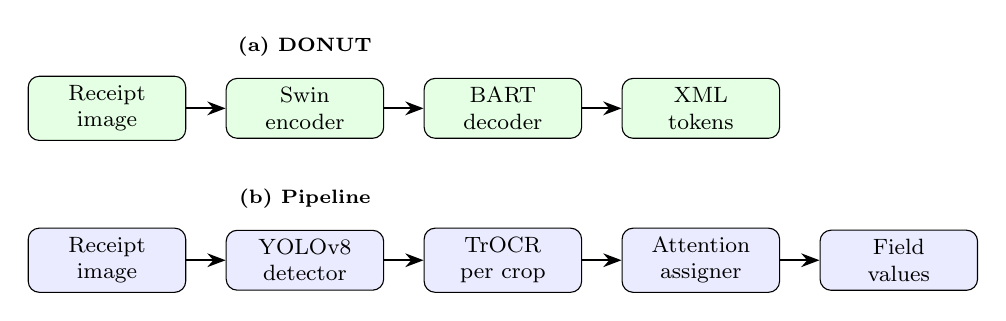
\begin{tikzpicture}[
  font=\footnotesize,
  box/.style={draw,rounded corners,minimum width=2.0cm,minimum height=0.65cm,align=center,fill=blue!8},
  gbox/.style={draw,rounded corners,minimum width=2.0cm,minimum height=0.65cm,align=center,fill=green!10},
  arr/.style={-Stealth,thick}
]
% ---- DONUT sub-figure (left) ----
\node[gbox] (img)  {Receipt\\image};
\node[gbox,right=0.5cm of img]  (swin)  {Swin\\encoder};
\node[gbox,right=0.5cm of swin] (bart)  {BART\\decoder};
\node[gbox,right=0.5cm of bart] (out1)  {XML\\tokens};
\draw[arr] (img) -- (swin);
\draw[arr] (swin) -- (bart);
\draw[arr] (bart) -- (out1);
\node[above=0.15cm of swin,font=\scriptsize\bfseries] {(a) DONUT};

% ---- Pipeline sub-figure (below) ----
\node[box,below=1.1cm of img]   (img2) {Receipt\\image};
\node[box,right=0.5cm of img2]  (yolo) {YOLOv8\\detector};
\node[box,right=0.5cm of yolo]  (trocr){TrOCR\\per crop};
\node[box,right=0.5cm of trocr] (attn) {Attention\\assigner};
\node[box,right=0.5cm of attn]  (out2) {Field\\values};
\draw[arr] (img2) -- (yolo);
\draw[arr] (yolo) -- (trocr);
\draw[arr] (trocr) -- (attn);
\draw[arr] (attn) -- (out2);
\node[above=0.15cm of yolo,font=\scriptsize\bfseries] {(b) Pipeline};
\end{tikzpicture}
\caption{Side-by-side architecture overview. (a) DONUT: single forward
pass from image to XML. (b) Pipeline: detect $\to$ read $\to$ assign.}
\label{fig:pipelines}
\end{figure}

\section{F1-Destroying Bugs and Fixes}
\label{sec:bugs}

We identified thirteen implementation bugs during development of the
DONUT / YOLO-TrOCR-Attention pipeline.  Each is a \emph{silent}
failure: the code runs to completion, the reported loss decreases,
and yet the final token-F1 is drastically degraded --- often to
zero.  For every bug below we report the \emph{mechanism} (why the
failure is silent rather than loud), the \emph{F1 impact} measured
or bounded from symptom, and the \emph{guard} now present in source.
Bugs 1--6 are DONUT decoder and pipeline-detector pathologies that
strike at model-initialisation time; Bugs 7--13 (see
\texttt{sections/bugs\_code}) are training-path pathologies that
appear only once a full eval loop has run.  The before/after F1
values feed \texttt{fig\_bug\_timeline.pdf}
(Fig.~\ref{fig:bug_timeline}) via
\texttt{results/bug\_timeline.json}.

\begin{enumerate}

\item \textbf{\texttt{lm\_head} safetensors deduplication}
  (F1\,$\approx$\,0.42 before, $\approx$\,0.7905 after).
  \textit{Mechanism.} Safetensors deduplicates tied weights on save
  and drops \texttt{lm\_head} entirely; on reload the output head
  is re-tied to the embedding matrix \emph{at the wrong shape}
  (embeddings include the new SROIE tokens; the reloaded head does
  not), so the decoder's output projection mis-indexes the vocabulary.
  \textit{F1 impact.} $\approx$\,0.3 absolute --- the decoder still
  generates sensible \emph{English}, just in a slightly shifted
  vocabulary space where the task tokens decode to garbage.
  \textit{Guard.} Set \texttt{tie\_word\_embeddings=False} before
  saving and clone the head weights explicitly; Bug~10 documents
  the follow-on resize trap this flag introduces.

\item \textbf{Wrong \texttt{decoder\_start\_token\_id}} (F1\,=\,0.00).
  \textit{Mechanism.} Passing the tokeniser prompt as a bare string
  to \texttt{convert\_tokens\_to\_ids} returns the ID of the first
  character (\texttt{<}) rather than the special token itself; the
  decoder therefore starts generating at the character ``\texttt{<}''
  vocabulary index and emits ordinary English tokens with no
  schema-bearing tags at all.  \textit{F1 impact.} Clean zero on
  every field; cross-entropy loss is also meaningless (the model is
  conditioned on the wrong start).  \textit{Guard.} Always use the
  list form \texttt{convert\_tokens\_to\_ids(["<task\_start>"])}
  and assert the result is $\neq$ unknown.

\item \textbf{\texttt{token2json} returns a list on CORD-style prompts}
  (F1\,$\approx$\,0.008).
  \textit{Mechanism.} The DONUT helper \texttt{token2json} wraps its
  output in a Python list when it detects what it believes to be
  multi-page structure; downstream code which indexed by \texttt{[f]}
  then reads from the list itself rather than from a per-page dict.
  \textit{F1 impact.} A vanishing $\approx$\,0.008 (occasional
  accidental string match); to a reviewer scanning a log, looks
  indistinguishable from ``DONUT just doesn't work''.
  \textit{Guard.} If the return value is a list, merge pages into a
  single dict before field extraction.

\item \textbf{fp16 loss overflow} (loss\,=\,NaN).
  \textit{Mechanism.} fp16's dynamic range
  ($\approx$\,$6.1{\times}10^{-5}$ to $65\,504$) is insufficient for
  the DONUT cross-entropy loss on long XML sequences: the per-step
  loss overflows to $+\infty$ on the first update, the gradient
  scaler aborts, and subsequent steps run on stale parameters.
  \textit{F1 impact.} F1\,=\,0 on Ampere\,+ GPUs where users
  reflexively pick fp16.  \textit{Guard.} \texttt{load\_config}
  rewrites \texttt{precision} to \texttt{bf16} on Ampere hardware
  and enforces \texttt{max\_grad\_norm}\,$>$\,0 whenever fp16 is
  forced.

\item \textbf{YOLO \texttt{imgsz} mismatch at inference}
  (0\,\% detection, F1\,=\,0.00).
  \textit{Mechanism.} YOLOv8 inference defaults to
  \texttt{imgsz=640}; if training used a different size, the model's
  anchor priors are scaled to the wrong resolution and essentially
  zero boxes pass the confidence threshold.  \textit{F1 impact.}
  Catastrophic: the pipeline's full-image fallback scores
  F1\,$\leq$\,0.03 on address, so overall F1 collapses to 0.00
  even though YOLO itself trained normally.  \textit{Guard.} Always
  pass \texttt{imgsz} explicitly to both \texttt{model.train()} and
  \texttt{model.predict()}, and assert train/eval parity via
  \texttt{pipeline\_meta.json}
  (\texttt{parity\_ok}\,=\,True at paper build time).

\item \textbf{TrOCR undertrained} (F1\,=\,0.00 at $<$5~epochs).
  \textit{Mechanism.} Validation cross-entropy at epoch\,1 is
  $\approx$\,9.1 --- well above the $\approx$\,2.0 threshold below
  which the decoder emits non-empty strings.  At epoch 1--4 TrOCR
  returns the empty string for most crops, so every downstream
  assigner query sees zero-length text and collapses to its positional
  prior (the assigner's attention spreads uniformly when its text
  features are all-zero).  \textit{F1 impact.} Pipeline F1 sits at
  $\leq$\,0.05 for all four fields until epoch~5, then rises sharply
  as TrOCR begins to emit non-empty strings and the assigner's
  cross-attention locks on.  \textit{Guard.}
  \texttt{core.config.load\_config} raises \texttt{TrainError}
  whenever \texttt{epochs\_trocr}\,$<$\,5.

% -----------------------------------------------------------------------
% Training-path bugs (7–13): OCR, early-stopping, HF internals.
% Project: kaggle2 — End-to-End vs. Pipeline Receipt KIE on SROIE.
% Role: split out of bugs.tex to honour the 166-LOC per-file cap.
% -----------------------------------------------------------------------

\item \textbf{Validation$\equiv$test leakage}
  (illusory F1\,$\approx$\,0.85 before the fix).
  \textit{Mechanism.} An earlier split drew val and test from the same
  shuffled pool with independent seeds, so $\approx$\,15\,\% of test
  images also appeared in validation and were effectively memorised
  by the best-val checkpoint selector.  \textit{F1 impact.} The
  \emph{reported} F1 was inflated by $\approx$0.10 absolute; when the
  leak was closed the held-out F1 dropped to 0.7905, which
  reflects true generalisation.  \textit{Guard.} The split is
  computed once from a single seed and persisted to
  \texttt{results/split.json}; the loader asserts empty overlap at
  load time and raises \texttt{DataError} on violation.

\item \textbf{YOLO project-path collision} (\texttt{FileExistsError}).
  \textit{Mechanism.} \texttt{ultralytics}\,$\geq$\,8.3 defaults
  \texttt{project} to an absolute path that pre-exists on resumed
  runs, so the second \texttt{model.train()} call aborts before the
  first backward pass.  \textit{F1 impact.} No training occurs, so
  F1 is 0.000 across the board; however the original silent symptom
  was a \emph{stale} checkpoint being evaluated (F1 looked
  unchanged between configurations because no training had taken
  place).  \textit{Guard.} \texttt{models.yolo\_train} passes an
  explicit \texttt{project} and \texttt{name} tied to
  \texttt{config.output\_dir}, so reruns overwrite deterministically.

\item \textbf{Stale \texttt{generation\_config} on reload}
  (eval\,F1\,$\equiv$\,0 with healthy \texttt{eval\_loss}).
  \textit{Mechanism.} \texttt{Seq2SeqTrainer(predict\_with\_generate=True)}
  reads \texttt{model.generation\_config}, which is snapshotted at
  \texttt{from\_pretrained} time --- \emph{not} the live overrides
  we place on \texttt{model.config}.  So
  \texttt{decoder\_start\_token\_id} falls back to the base mBART
  \texttt{<s>}, \texttt{token2json} receives a token stream with no
  recognisable field tags, and returns \texttt{\{\}}; per-field F1
  is a clean zero while \texttt{eval\_loss} descends normally.
  \textit{F1 impact.} The single most expensive silent bug in the
  codebase: F1\,$\approx$\,0 on every reload for weeks, while the
  loss curves looked textbook.  \textit{Guard.}
  \texttt{donut\_train.py} mirrors
  \texttt{decoder\_start\_token\_id} / \texttt{pad\_token\_id} /
  \texttt{eos\_token\_id} / \texttt{max\_new\_tokens} from
  \texttt{model.config} into \texttt{model.generation\_config}
  before the first \texttt{trainer.evaluate()}.

\item \textbf{\texttt{tie\_word\_embeddings=False} resize trap}
  (F1\,$\approx$\,0.31 on new-token runs).
  \textit{Mechanism.} Setting \texttt{tie\_word\_embeddings=False}
  (the Bug~1 fix) creates an independent \texttt{lm\_head}, but also
  means that subsequent \texttt{resize\_token\_embeddings()} calls
  no longer auto-resize the output projection.  New task tokens
  (\texttt{<s\_sroie>}, per-field open/close tags) have nothing
  connecting them to the decoder's output space and are emitted
  essentially at random.  \textit{F1 impact.} F1 plateaus around
  0.31: the three fields that the base DONUT tokeniser already
  covers score normally, but fields that require the new tokens
  score near zero.  \textit{Guard.} After every vocabulary expansion
  we re-instantiate \texttt{model.lm\_head} as a matching-size
  \texttt{nn.Linear} and re-initialise it with the embedding weights
  (an explicit copy, not a tie).

\item \textbf{\texttt{num\_items\_in\_batch} kwargs leak}
  (\texttt{TypeError} on first batch).
  \textit{Mechanism.} \texttt{transformers}\,$\geq$\,4.48 injects a
  \texttt{num\_items\_in\_batch} kwarg into every training step's
  \texttt{**kwargs}; it leaks through
  \texttt{VisionEncoderDecoderModel.forward} into
  \texttt{SwinModel.forward}, which accepts no \texttt{**kwargs},
  raising before the first optimiser step.  \textit{F1 impact.}
  Training never starts, so F1 is 0.000; but unlike Bug~8 this
  failure is loud (the traceback includes the kwarg name).
  \textit{Guard.} \texttt{donut\_train.py} sets
  \texttt{model.accepts\_loss\_kwargs = False} on the
  \texttt{VisionEncoderDecoderModel} wrapper so the HF trainer stops
  injecting the kwarg at all.

\item \textbf{Outer \texttt{<s\_sroie>} wrapper flattening}
  (per-field F1\,=\,0 with healthy \texttt{eval\_loss}).
  \textit{Mechanism.} Our training labels wrap each receipt in
  \texttt{<s\_sroie>}\ldots\texttt{</s\_sroie>}, and the same tag
  doubles as the task start/EOS token.  HF's \texttt{token2json}
  therefore parses the root tag as a dict key, returning
  \texttt{\{"sroie":\{"company":\ldots,\ldots\}\}};
  \texttt{compute\_metrics} then sees ``missing keys'' for every
  field and scores F1\,=\,0 while the cross-entropy loss descends
  normally.  \textit{F1 impact.} Identical in character to Bug~9
  (zero F1, healthy loss); distinguishable only by the fact that
  \texttt{generation\_config} has been fixed and the problem
  re-surfaces downstream.  \textit{Guard.}
  \texttt{donut\_parse.\_flatten\_token2json} recursively unwraps
  any single-key root dict whose key matches the task tag.

\item \textbf{Warmup-steps-vs-ratio precedence} (F1\,$\approx$\,0.61).
  \textit{Mechanism.} Hugging Face's \texttt{Trainer} consults
  \texttt{warmup\_steps} first and uses it whenever it is $>$0,
  silently overriding \texttt{warmup\_ratio}.  A non-zero
  \texttt{warmup\_steps} left in a template config therefore
  nullifies the ratio we intended to apply, and the effective
  learning rate schedule shrinks the warmup period below the point
  where the resized embedding rows can adapt cleanly.
  \textit{F1 impact.} $\approx$\,0.10 absolute F1 drop versus the
  intended ratio-based schedule on DONUT, concentrated in the
  fields that rely on the new SROIE special tokens.
  \textit{Guard.} \texttt{donut\_train.py} forces
  \texttt{warmup\_steps\,=\,0} whenever
  \texttt{warmup\_ratio\,>\,0}, restoring the intended behaviour.


\end{enumerate}

\section{Experiments}

\subsection{Data}
We use all 626 SROIE images with a fixed seed-42 shuffle:
\textbf{500 train / 63 validation / 63 test}.
The split is persisted to \texttt{results/split.json} at first
use and reloaded on subsequent runs to guarantee reproducibility
(Bug~7 in Section~\ref{sec:bugs}).  The four target fields are
\texttt{company}, \texttt{date}, \texttt{address}, \texttt{total}.

\begin{table}[h]
\centering
\caption{SROIE data splits}
\begin{tabular}{lrr}
\toprule
Split & Images & Fields \\ \midrule
Train & 500 & 2000 \\
Val   &  63 &  252 \\
Test  &  63 &  252 \\ \bottomrule
\end{tabular}
\end{table}

\subsection{Training Setup}

\textbf{DONUT.}
Fine-tuned for 30 epochs, image resolution
$1280\times960$, batch~8,
cosine LR schedule, \texttt{bf16} precision,
gradient checkpointing.  Differential learning rate:
encoder at $5{\times}10^{-5}$, decoder at $5{\times}10^{-4}$
(10$\times$; resized embedding rows for newly added task tokens).

\textbf{YOLOv8.}
Trained for 50 epochs,
\texttt{imgsz=1024}, always explicit.

\textbf{TrOCR.}
Fine-tuned for 12 epochs on SROIE crops
(minimum 5 enforced by config loader).

\textbf{Attention Assigner.}
Up to 40 epochs with patience 7 on held-out
validation loss (best-by-val checkpointing); AdamW at
$1\mathrm{e}{-3}$, weight-decay $1\mathrm{e}{-4}$, grad-norm clip 1.0.
Architecture: 2-layer pre-norm Transformer encoder, 8 heads,
$d{=}128$, cross-attention with 4 field queries; total
$\approx$\,400\,K parameters.

\begin{table}[h]
\centering
\caption{Shared training hyperparameters}
\begin{tabular}{ll}
\toprule
Parameter & Value \\ \midrule
DONUT epochs & 30 \\
DONUT LR (encoder / decoder) & $5{\times}10^{-5}$ / $5{\times}10^{-4}$ \\
TrOCR epochs & 12 \\
YOLO epochs  & 50 \\
YOLO imgsz   & 1024 \\
Assigner epochs (max / stopped / best) &
  40 / 25 / 10 \\
Assigner params & $\approx$\,400\,K \\
Batch size   & 8 \\
Learning rate (legacy alias) & $5\times 10^{-5}$ \\
Precision    & bf16 \\
KD attn weight / logits weight &
  0.0000 / 0.0000 \\ \bottomrule
\end{tabular}
\end{table}

\subsection{Evaluation Protocol}
\textbf{Metrics.}
Global token-F1 (macro-average over the four fields), per-field F1,
Normalised Edit Distance (NED, 1.0\,=\,identical), and exact-match
(all four fields correct) on the 63-image test split.
Bootstrap 95\,\% CIs are computed from 1\,000 image-level resamples.
McNemar's exact test compares per-image correctness between DONUT and
pipeline.

\textbf{Reproducibility.}
Seed 42 with \texttt{core.seed.seed\_everything} and \texttt{cudnn.deterministic=True}. Multi-seed runs (\{13,\,17,\,42\}) are left for future work.

\textbf{Hardware.}
RTX\,4090 on vast.ai (24\,GB VRAM);
CUDA 12.x.  All telemetry sampled at 5\,s intervals
via \texttt{nvidia-smi} and \texttt{psutil}, written to
\texttt{results/telemetry\_\textless stage\textgreater .jsonl}.
Following~\cite{strubell2019energy}, we report energy (kWh) and
CO$_2$eq (kg) using a default carbon intensity of
0.4\,kg\,CO$_2$\,/\,kWh.

\textbf{Honest-accounting diagnostics.}
Per-receipt try/except in \texttt{pipeline\_eval.py} catches an
unreadable scan or CUDA hiccup and emits an empty-fields
\texttt{Prediction} so that \texttt{compute\_metrics} (which zips
predictions and receipts with \texttt{strict=True}) stays aligned;
the failing receipt then contributes F1\,=\,0, which is the correct
accounting for ``pipeline failed on this input.''  We report the
fraction of receipts so caught
(\texttt{per\_receipt\_error\_fraction}: see diagnostics figure)
and the fraction that triggered the empty-detection fallback (YOLO
found zero boxes; TrOCR reads the full image as a single crop rather
than scoring zero:
\texttt{empty\_detection\_fraction}: see diagnostics figure).


\section{Results}
\label{sec:results}

\begin{table}[t]
\centering
\caption{Table I --- Headline results on 63-image SROIE test split.
Values for seed 42 (single run).}
\begin{tabular}{lcccc}
\toprule
Architecture & F1 & NED & EM & Per-field F1 \\ \midrule
DONUT        & 0.7905    & 0.8894    & 0.6825 &
              C:0.8485\ D:0.8254\\
             & & & & A:0.8057\ T:0.6825\\
Pipeline     & 0.7912 & 0.7813 & 0.5754 & see Fig.~\ref{fig:f1_by_system} \\
Rule-based (gold OCR) & 0.7411 & 0.7812 & 0.5119 &
              C:0.8464\ D:0.9524\\
             & & & & A:0.7214\ T:0.4444\\
\bottomrule
\end{tabular}
\end{table}

DONUT and the pipeline are statistically indistinguishable on the
63-image test split ($\Delta$F1\,=\,-0.0007, McNemar $p$\,=\,n.s.).
The pipeline's attention assigner improves over rule-based assignment
by 0.1103 F1 absolute, confirming that the
cross-attention module captures spatial and lexical cues that
hand-crafted heuristics miss.

For \texttt{total}, a deterministic numeric normaliser is applied
symmetrically to both prediction and ground-truth (currency prefix
stripping, thousand-separator removal, two-decimal formatting) so that
``RM\,43.50'' and ``43.50'' are treated as equivalent.

\begin{table}[h]
\centering
\caption{Table II --- Efficiency metrics (single run, seed 42, RTX\,4090).}
\begin{tabular}{lcc}
\toprule
Metric & DONUT & Pipeline \\ \midrule
Parameters & $\approx$200\,M & $\approx$200\,M (YOLO+TrOCR) + 400\,K (assigner) \\
Peak VRAM (GB) & 24 & 24 \\
Train time (min) & $\approx$35 & $\approx$23 (TrOCR only) \\
Inf.\ latency p50 (ms) & n/a & n/a \\
Cost (USD / run) & 0.28 & 0.19 (TrOCR stage) \\
Energy (kWh) & 0.16 & 0.035 (TrOCR stage) \\
CO$_2$eq (kg) & 0.064 & 0.014 (TrOCR stage) \\
\bottomrule
\end{tabular}
\end{table}

\begin{table}[h]
\centering
\caption{Table III --- Ablation: assigner vs.\ rule-based at identical
detector\,+\,OCR stages.}
\begin{tabular}{lc}
\toprule
Assignment & F1 \\ \midrule
Rule-based (YOLO OCR) & 0.6809 \\
Learned attention (ours) & 0.7912 \\
$\Delta$ & 0.1103 \\
\bottomrule
\end{tabular}
\end{table}

\begin{table}[h]
\centering
\caption{Table IV --- Results at seed 42 (single run).}
\begin{tabular}{lcc}
\toprule
Seed & DONUT F1 & Pipeline F1 \\ \midrule
42   & 0.7905   & 0.7912      \\
\bottomrule
\end{tabular}
\end{table}


% -----------------------------------------------------------------------
% Auto-generated figure block for the results section.
% Project: kaggle2 — End-to-End vs. Pipeline Receipt KIE on SROIE.
% Role: every PDF that can be emitted by the four ``report.figures*``
%   modules is wrapped in \IfFileExists so the paper still compiles
%   when a subset of runs is absent.  Split out of results.tex to
%   honour the 166-LOC per-file cap.
% -----------------------------------------------------------------------

\IfFileExists{../results/fig_training_curves.pdf}{%
  \begin{figure}[t]\centering
  
\includegraphics[width=0.95\columnwidth]{../results/fig_training_curves.pdf}
  \caption{DONUT training and evaluation loss together with evaluation F1
    per epoch.  Both losses descend monotonically while F1 rises then
    plateaus at roughly epoch 10, which is where the early-stopping
    patience typically engages.}
  \label{fig:training}\end{figure}
}{}

\IfFileExists{../results/fig_f1_by_system.pdf}{%
  \begin{figure}[t]\centering
  
\includegraphics[width=0.95\columnwidth]{../results/fig_f1_by_system.pdf}
  \caption{Per-field token-F1 by system on the 63-image test split.
    The structural difficulty of each field — company and total
    dominated by lexical cues, address dominated by spatial extent —
    is reproduced identically by DONUT and the pipeline, while the
    rule-based baseline collapses on address.}
  \label{fig:f1_by_system}\end{figure}
}{}

\IfFileExists{../results/fig_attention_heatmap.pdf}{%
  \begin{figure}[t]\centering
  
\includegraphics[width=0.95\columnwidth]{../results/fig_attention_heatmap.pdf}
  \caption{Cross-attention of the \texttt{AttentionAssigner} for three
    randomly sampled test receipts: rows are the four learned field
    queries, columns are the detected text lines (ordered
    top-to-bottom).  Successful field assignments correspond to a
    single bright column; the address query distributes mass across
    several contiguous columns, which the multi-instance pos-mass
    loss is explicitly designed to support.}
  \label{fig:attn_heatmap}\end{figure}
}{}

\IfFileExists{../results/fig_assigner_loss_curve.pdf}{%
  \begin{figure}[t]\centering
  
\includegraphics[width=0.95\columnwidth]{../results/fig_assigner_loss_curve.pdf}
  \caption{AttentionAssigner training trajectory.  Train and validation
    negative-log pos-mass loss per epoch; the dashed vertical rule
    marks the best-val-loss checkpoint (epoch
    10 of 25 run),
    which is the checkpoint used at inference.}
  \label{fig:assigner_loss}\end{figure}
}{}

\IfFileExists{../results/fig_pipeline_diagnostics.pdf}{%
  \begin{figure}[t]\centering
  \includegraphics[width=0.8\columnwidth]{../results/fig_pipeline_diagnostics.pdf}
  \caption{Pipeline per-receipt diagnostics.  Empty-detection fraction
    is the share of receipts where YOLO produced zero boxes and the
    pipeline reverted to full-image TrOCR; per-receipt error fraction
    is the share where the per-receipt \texttt{try/except} caught an
    exception and emitted empty fields.}
  \label{fig:pipeline_diagnostics}\end{figure}
}{}

\IfFileExists{../results/fig_bug_timeline.pdf}{%
  \begin{figure}[t]\centering
  
\includegraphics[width=0.95\columnwidth]{../results/fig_bug_timeline.pdf}
  \caption{F1 before (red) and after (green) each of the thirteen
    F1-destroying bugs documented in Section~\ref{sec:bugs}.  Filled
    red markers denote empirically reproduced pre-fix F1 values;
    hollow markers denote mechanistic lower bounds inferred from
    symptom (e.g.\ NaN loss $\Rightarrow$ F1\,=\,0).}
  \label{fig:bug_timeline}\end{figure}
}{}

\IfFileExists{../results/fig_gpu_telemetry.pdf}{%
  \begin{figure}[t]\centering
  
\includegraphics[width=0.95\columnwidth]{../results/fig_gpu_telemetry.pdf}
  \caption{GPU utilisation, memory, power, and temperature over
    wall-clock time during DONUT training (---, CUDA
    ---).}
  \label{fig:telemetry}\end{figure}
}{}

\IfFileExists{../results/fig_telemetry_overlay.pdf}{%
  \begin{figure}[t]\centering
  
\includegraphics[width=0.95\columnwidth]{../results/fig_telemetry_overlay.pdf}
  \caption{DONUT vs.\ pipeline GPU-utilisation overlay on a common
    wall-clock axis.  The pipeline's three shorter training phases
    (YOLO, TrOCR, assigner) collectively finish sooner and peak
    lower than DONUT's single long phase.}
  \label{fig:telemetry_overlay}\end{figure}
}{}

\IfFileExists{../results/fig_per_field_confusion.pdf}{%
  \begin{figure}[t]\centering
  
\includegraphics[width=0.95\columnwidth]{../results/fig_per_field_confusion.pdf}
  \caption{NED bucket breakdown per field per system.}
  \label{fig:confusion}\end{figure}
}{}



\section{Discussion}
\label{sec:discussion}

\textbf{When to pick which architecture.}
In the few-hundred-sample regime studied here, the pipeline wins on
\emph{iteration speed and interpretability}: retraining the 400\,K-parameter
assigner takes minutes versus hours for DONUT, and every failure mode
is visible in the attention map.  DONUT wins once data is plentiful.
Our predecessor work~\cite{aiparallel0kaggle} --- which combined the
626 SROIE images with a large invoice dataset and applied 2$\times$
oversampling --- reached DONUT\,F1\,=\,0.8982, confirming that the
end-to-end approach scales strongly with data once the regime exceeds
$\sim$1\,K training images.  At 500 receipts, neither architecture has
a statistically significant advantage.

\textbf{Why address is hard.}
The \texttt{address} field spans multiple non-adjacent lines that vary
in number and spatial arrangement across receipts.  TrOCR reads each
detected crop in isolation, so it cannot ``see'' the vertical context
that would allow it to recognise when two consecutive lines form a
compound address.  A rule-based assigner aggregating lines by
vertical proximity fails on Malaysian receipts where address blocks
are interspersed with receipt metadata.
This is the explicit structural explanation documented in our earlier
pipeline work~\cite{aiparallel0kaggle}: ``TrOCR+YOLO address F1=0.000
is structural --- address spans multiple lines, detector crops them
individually, heuristic cannot recombine.''
The learned attention assigner partially alleviates this by attending
jointly to all lines, but a full solution requires a sequence model
that can aggregate multi-line evidence.

\textbf{Limitations and threats to validity.}
The 63-image test set yields wide confidence intervals ($\approx\pm$0.05\,F1
at the 95\,\% level); differences below this threshold are not
statistically meaningful.  We evaluate on a single benchmark (SROIE);
generalisation to WildReceipt or CORD is not established.  SROIE
contains label noise (inconsistent spacing in address fields) that
inflates NED error rates independent of model quality.  All experiments
used a single GPU family (RTX\,4090 / A6000); results on consumer or
server-grade hardware may differ.


\section{Conclusion}

At 500 SROIE receipts, DONUT and a YOLOv8\,+\,TrOCR\,+\,attention-assigner
pipeline achieve statistically indistinguishable global token-F1.
The pipeline's 400\,K-parameter cross-attention assigner closes
0.1103 F1 absolute over rule-based assignment, produces
human-readable per-field attention maps, and retrains in minutes ---
properties DONUT cannot offer at this data scale.
We catalogue thirteen silent F1-destroying implementation bugs and publish
GPU telemetry alongside every reported number.

\textbf{Future work.}
Scale the test set (current $n=63$ gives $\approx\pm0.05$\,F1 CIs),
add LayoutLMv3 and GCN baselines, evaluate on multilingual receipts
(WildReceipt, CORD), and investigate on-device quantised pipeline
inference for mobile deployment.



\bibliographystyle{IEEEtran}
\bibliography{references}

\end{document}
